%%%%%%%%%%%%%%%%%%%%%%%%%%%%%%%%%%%%%%%%%
% Stylish Article
% LaTeX Template
% Version 2.1 (1/10/15)
%
% This template has been downloaded from:
% http://www.LaTeXTemplates.com
%
% Original author:
% Mathias Legrand (legrand.mathias@gmail.com)
% With extensive modifications by:
% Vel (vel@latextemplates.com)
% Optimized for Ferris State University by Dr. Clifton Franklund
%
% License:
% CC BY-NC-SA 3.0 (http://creativecommons.org/licenses/by-nc-sa/3.0/)
%
%%%%%%%%%%%%%%%%%%%%%%%%%%%%%%%%%%%%%%%%%

%----------------------------------------------------------------------------------------
%	PACKAGES AND OTHER DOCUMENT CONFIGURATIONS
%----------------------------------------------------------------------------------------

\documentclass[fleqn,10pt]{SelfArx}\usepackage[]{graphicx}\usepackage[]{color}
%% maxwidth is the original width if it is less than linewidth
%% otherwise use linewidth (to make sure the graphics do not exceed the margin)
\makeatletter
\def\maxwidth{ %
  \ifdim\Gin@nat@width>\linewidth
    \linewidth
  \else
    \Gin@nat@width
  \fi
}
\makeatother

\definecolor{fgcolor}{rgb}{0.345, 0.345, 0.345}
\newcommand{\hlnum}[1]{\textcolor[rgb]{0.686,0.059,0.569}{#1}}%
\newcommand{\hlstr}[1]{\textcolor[rgb]{0.192,0.494,0.8}{#1}}%
\newcommand{\hlcom}[1]{\textcolor[rgb]{0.678,0.584,0.686}{\textit{#1}}}%
\newcommand{\hlopt}[1]{\textcolor[rgb]{0,0,0}{#1}}%
\newcommand{\hlstd}[1]{\textcolor[rgb]{0.345,0.345,0.345}{#1}}%
\newcommand{\hlkwa}[1]{\textcolor[rgb]{0.161,0.373,0.58}{\textbf{#1}}}%
\newcommand{\hlkwb}[1]{\textcolor[rgb]{0.69,0.353,0.396}{#1}}%
\newcommand{\hlkwc}[1]{\textcolor[rgb]{0.333,0.667,0.333}{#1}}%
\newcommand{\hlkwd}[1]{\textcolor[rgb]{0.737,0.353,0.396}{\textbf{#1}}}%

\usepackage{framed}
\makeatletter
\newenvironment{kframe}{%
 \def\at@end@of@kframe{}%
 \ifinner\ifhmode%
  \def\at@end@of@kframe{\end{minipage}}%
  \begin{minipage}{\columnwidth}%
 \fi\fi%
 \def\FrameCommand##1{\hskip\@totalleftmargin \hskip-\fboxsep
 \colorbox{shadecolor}{##1}\hskip-\fboxsep
     % There is no \\@totalrightmargin, so:
     \hskip-\linewidth \hskip-\@totalleftmargin \hskip\columnwidth}%
 \MakeFramed {\advance\hsize-\width
   \@totalleftmargin\z@ \linewidth\hsize
   \@setminipage}}%
 {\par\unskip\endMakeFramed%
 \at@end@of@kframe}
\makeatother

\definecolor{shadecolor}{rgb}{.97, .97, .97}
\definecolor{messagecolor}{rgb}{0, 0, 0}
\definecolor{warningcolor}{rgb}{1, 0, 1}
\definecolor{errorcolor}{rgb}{1, 0, 0}
\newenvironment{knitrout}{}{} % an empty environment to be redefined in TeX

\usepackage{alltt} % Document font size and equations flushed left
\usepackage[english]{babel}         % Specify a different language here - english by default
\usepackage{lipsum}                 % Required to insert dummy text. To be removed otherwise
\usepackage{fancyhdr}               % Required to put the logo on the top of the first page
\usepackage{float}                  % Extra help with figures and tables
\usepackage{caption}                % Helps to format captions
\captionsetup[table]{skip=3pt}      % Spacing after caption
\usepackage{enumitem}               % Tightening lists
\setlist[itemize]{itemsep=0mm}      % Tightening lists
\usepackage[style=authoryear,doi=false,isbn=false,url=false,natbib=true,backend=biber]{biblatex}
\bibliography{references}           % Point to the bibtex bibliography file

%----------------------------------------------------------------------------------------
%	COLUMNS
%----------------------------------------------------------------------------------------

\setlength{\columnsep}{0.55cm}      % Distance between the two columns of text
\setlength{\fboxrule}{0.75pt}       % Width of the border around the abstract

%----------------------------------------------------------------------------------------
%	COLORS
%----------------------------------------------------------------------------------------

\definecolor{color1}{RGB}{0,0,0}         % Color of the article title
\definecolor{color2}{RGB}{255,255,255}   % Section heading text color
\definecolor{color3}{RGB}{178,34,34}     % Color of the boxes behind the abstract and headings

%----------------------------------------------------------------------------------------
%	HYPERLINKS
%----------------------------------------------------------------------------------------

\usepackage{hyperref}               % Required for hyperlinks
\hypersetup{hidelinks,colorlinks,breaklinks=true,urlcolor=color3,citecolor=color3,linkcolor=color3,bookmarksopen=false,pdftitle={Title},pdfauthor={Author}}

%----------------------------------------------------------------------------------------
%	NO SECTION NUMBERS
%----------------------------------------------------------------------------------------
\setcounter{secnumdepth}{0}

%----------------------------------------------------------------------------------------
%	ARTICLE INFORMATION
%----------------------------------------------------------------------------------------

\JournalInfo{General Education Assessment}     % Report information
\Archive{Report 16(1) --- July 2016}           % Report identifier and date)

\PaperTitle{Meta-Analysis of Student Achievement on Natural Science FLO SCI1 in a 200-Level Biology Course} % Article title

\Authors{Dr. Clifton Franklund\textsuperscript{1}} % Authors
\affiliation{\textsuperscript{1}\textit{General Education Coordinator, Ferris State University}} % Author affiliation

\Keywords{Meta-Analysis --- Forest plot --- Natural Sciences --- Scientific concepts}
\newcommand{\keywordname}{Keywords} % Defines the keywords heading name

%----------------------------------------------------------------------------------------
%	ABSTRACT
%----------------------------------------------------------------------------------------

\Abstract{Lorem ipsum dolor sit amet, consectetur adipisicing elit, sed do eiusmod tempor incididunt ut labore et dolore magna aliqua. Ut enim ad minim veniam, quis nostrud exercitation ullamco laboris nisi ut aliquip ex ea commodo consequat. Duis aute irure dolor in reprehenderit in voluptate velit esse cillum dolore eu fugiat nulla pariatur. Excepteur sint occaecat cupidatat non proident, sunt in culpa qui officia deserunt mollit anim id est laborum.~}

%----------------------------------------------------------------------------------------
\IfFileExists{upquote.sty}{\usepackage{upquote}}{}
\begin{document}

\flushbottom % Makes all text pages the same height

\maketitle % Print the title and abstract box

\tableofcontents % Print the contents section

% Set up the first page to have the Ferris logo in the left
\fancypagestyle{firststyle}
{
	\fancyhf{}
	\fancyhead[L]{
\includegraphics[height=0.55cm]{./figure/logo.png}}
}
\thispagestyle{firststyle}


%----------------------------------------------------------------------------------------
%	INITIALIZE R FOR THIS DOCUMENT
%----------------------------------------------------------------------------------------








%----------------------------------------------------------------------------------------
%	ARTICLE CONTENTS
%----------------------------------------------------------------------------------------

\section{Introduction} % The \section*{} command stops section numbering
%\addcontentsline{toc}{section}{Introduction} % Adds this section to the table of contents

PUT THE INTRODUCTION TEXT HERE.

%------------------------------------------------

\section{Methods}
%\addcontentsline{toc}{section}{Methods} % Adds this section to the table of contents

\subsection{Collection of assessment data}
Student performance on the first lecture exam in a 200-level Biology course was analyzed. Individual student scores were collected using the new General Education Natural Sciences "scores" data workbook for thirteen semesters. Student scores were automatically converted to a rubric score by the workbook using the equivalencies shown in Table \ref{tab:convert}.

\begin{table}[hbt]
\caption{Conversion of percentages to rubric scores}
\centering
\begin{tabular}{c c c}
\textbf{Percent correct} & \textbf{Rubric} & \textbf{Interpretation}   \\
\hline
 0.0 to 49.9\%   &   0   &   Unsatisfactory                                \\
50.0 to 59.9\%   &   1   &   Beginning                                     \\
60.0 to 69.9\%   &   2   &   Developing                                    \\
70.0 to 84.9\%   &   3   &   Proficient                                    \\
85.0 to 100.0\%  &   4   &   Advanced                                      \\
\end{tabular}
\label{tab:convert}
\end{table}

These files all contain personally identifiable information (PII) and are, therefore, subject to FERPA regulations. For this reason, they are not directly shared. Instead, they are stored in a data folder in TracDat: Core Competency: Natural Sciences $\Rightarrow$ Assessment $\Rightarrow$ Proof of Concept.

\subsection{De-identification of student data}
Copies of the 13 data files were downloaded from TracDat. An R aggregator script was used to read the data from these data sheets and contatenate it into one dataset. Student names were removed and each student's entry was given a unique eight-digit identifier - the Record.Key. These keys may be used for longitudinal studies in the future. The algorithm used is kept in an encrypted site and shared with \textit{noone}. The de-identified dataset contains 973 student entries and is stored as a comma-delimited textfile (BIOL200Data.csv).

\subsection{Data provenance}
\paragraph{Location of public website files} \lipsum[1] % Dummy text

\paragraph{Citation of this work}
All of the de-identified data, analysis code, and documentation that constitute this report project may be freely used, modified, and shared. The code file, Gen\_Ed\_Report\_16-01.Rmd, is released under the \href{https://opensource.org/licenses/MIT}{MIT license}. The de-identified dataset, BIOL200Data.csv, is released under the Creative Commons \href{https://creativecommons.org/publicdomain/zero/1.0/}{CC0 license}. All documentation, including README.md, Codebook.md, and this report, are released under the Creative Commons \href{https://creativecommons.org/licenses/by/4.0/}{CC-BY} licence. Any questions, comments, or suggestions may be sent to \href{mailto:CliftonFranklund@ferris.edu}{Dr. Franklund}.

\paragraph{Session information}
The following information pertains to the session used to generate this report.
\begin{itemize}\raggedright
  \item R version 3.3.0 (2016-05-03), \verb|x86_64-apple-darwin13.4.0|
  \item Base packages: base, datasets, graphics, grDevices, grid,
    methods, stats, utils
  \item Other packages: car~2.1-2, dplyr~0.5.0, forestplot~1.5.1,
    Formula~1.2-1, gdata~2.17.0, ggplot2~2.1.0, Hmisc~3.17-4,
    knitr~1.13, lattice~0.20-33, magrittr~1.5, mice~2.25,
    moments~0.14, papeR~1.0-1, Rcpp~0.12.6, survival~2.39-5,
    weights~0.85, xtable~1.8-2
  \item Loaded via a namespace (and not attached):
    acepack~1.3-3.3, assertthat~0.1, chron~2.3-47, cluster~2.0.4,
    colorspace~1.2-6, data.table~1.9.6, DBI~0.4-1, evaluate~0.9,
    foreign~0.8-66, formatR~1.4, gmodels~2.16.2, gridExtra~2.2.1,
    gtable~0.2.0, gtools~3.5.0, latticeExtra~0.6-28, lme4~1.1-12,
    MASS~7.3-45, Matrix~1.2-6, MatrixModels~0.4-1, mgcv~1.8-13,
    minqa~1.2.4, munsell~0.4.3, nlme~3.1-128, nloptr~1.0.4,
    nnet~7.3-12, parallel~3.3.0, pbkrtest~0.4-6, plyr~1.8.4,
    quantreg~5.26, R6~2.1.2, RColorBrewer~1.1-2, rpart~4.1-10,
    scales~0.4.0, SparseM~1.7, splines~3.3.0, stringi~1.1.1,
    stringr~1.0.0, tibble~1.1, tools~3.3.0
\end{itemize}

\section{Results}
\lipsum[1]

\subsection{Structure of the report files}
\lipsum[1]

\subsection{Summary statistics}
This is just some random repeating text. This is just some random repeating text. This is just some random repeating text. This is just some random repeating text. This is just some random repeating text. This is just some random repeating text. This is just some random repeating text. This is just some random repeating text. This is just some random repeating text. This is just some random repeating text.

\begin{figure}[h]\centering

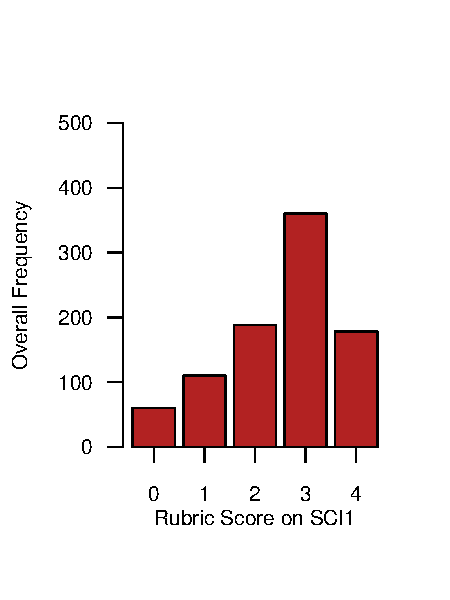
\includegraphics[width=\columnwidth,viewport = 0 20 216 240]{./figure/histogram}
\protect\caption{A histogram of the distribution of individual rubric score frequencies over all twelve semesters.}
\label{fig:histogram}
\end{figure}

The overall overall average rubric score for all 13 semesters was 2.54. The distribution of the rubrics scores is shown below.

\begin{figure}[h]\centering

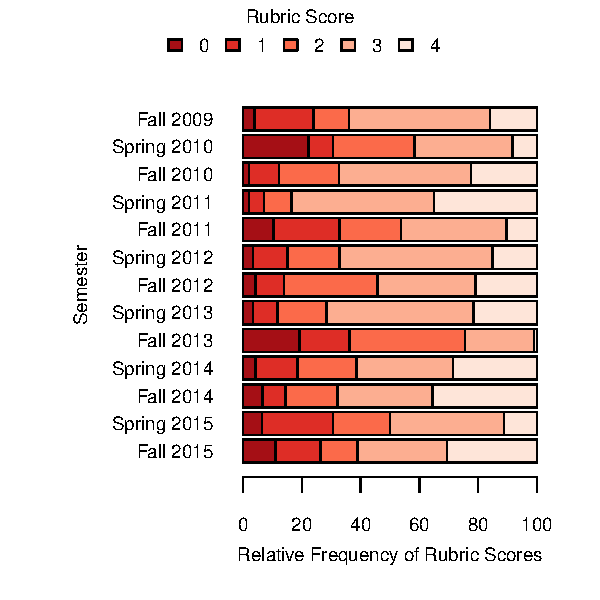
\includegraphics[width=\columnwidth,viewport = 30 0 288 288]{./figure/barplot}
\protect\caption{A barplot showing the distribution of rubric scores broken down by semester.}
\label{fig:barplot}
\end{figure}

\begin{center}
% latex table generated in R 3.3.0 by xtable 1.8-2 package
% Mon Aug 15 14:44:07 2016
\begin{table}[ht]
\centering
\caption{One-way ANOVA analysis of scores by semester} 
\label{tab:anova}
\begin{tabular}{lrrrrr}
  \hline
 & Df & Sum Sq & Mean Sq & F value & Pr($>$F) \\ 
  \hline
Semester & 12 & 142.74 & 11.89 & 9.85 & 0.0000 \\ 
  Residuals & 960 & 1159.22 & 1.21 &  &  \\ 
   \hline
\end{tabular}
\end{table}

\end{center}

\lipsum[1]
\subsection{Meta-analysis}
\begin{figure*}[htb]\centering % Using \begin{figure*} makes the figure take up the entire width of the page

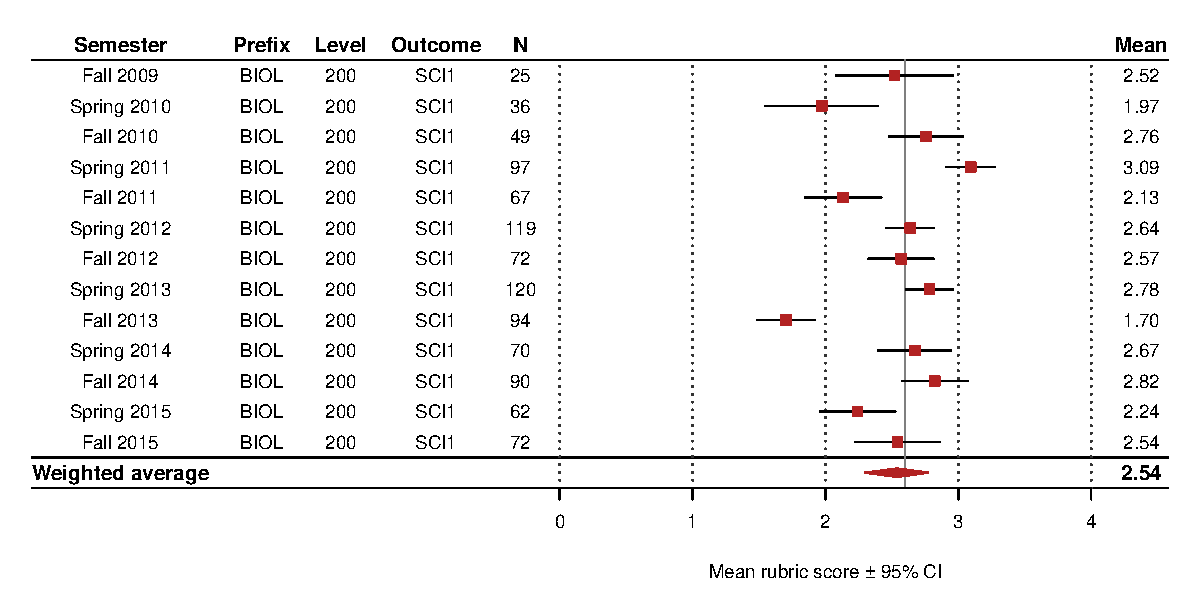
\includegraphics[width=\textwidth]{./figure/forest}
\protect\caption{A forest plot of the average scores for each semester with a weighted mean estimate for the entire period investigated. Error bars indicate the 95\% confidence intervals.}
\label{fig:forest.pdf}
\end{figure*}

\lipsum[1] % Dummy text
\lipsum[1]

\begin{equation}
\cos^3 \theta =\frac{1}{4}\cos\theta+\frac{3}{4}\cos 3\theta
\label{eq:refname2}
\end{equation}

\lipsum[1] % Dummy text

\begin{enumerate}[noitemsep] % [noitemsep] removes whitespace between the items for a compact look
\item First item in a list
\item Second item in a list
\item Third item in a list
\end{enumerate}

\begin{figure}[ht]\centering
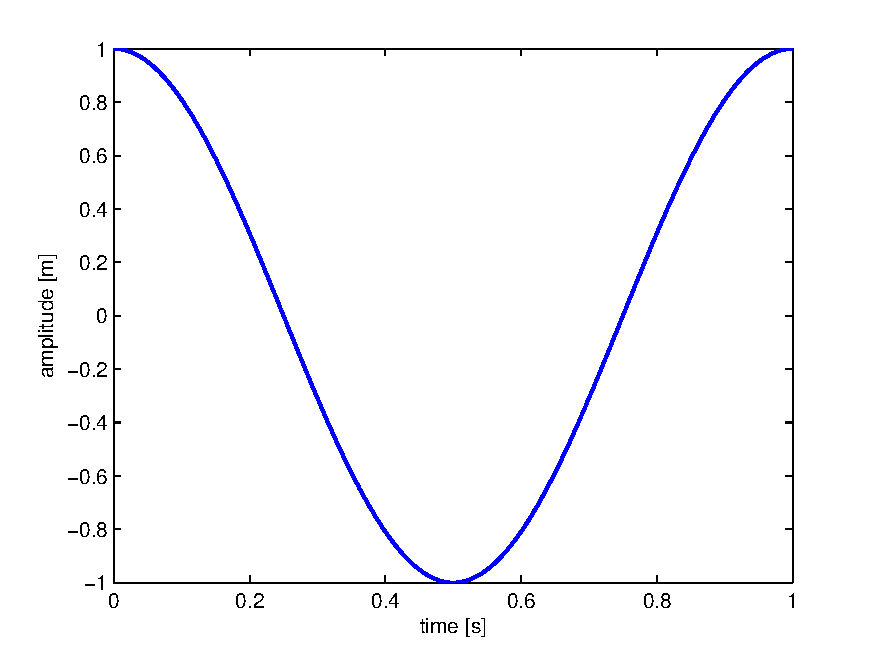
\includegraphics[width=\linewidth]{results}
\caption{In-text Picture}
\label{fig:results}
\end{figure}

Reference to Figure \ref{fig:results}.

%------------------------------------------------

\section{Discussion}
%\addcontentsline{toc}{section}{Results and Discussion} % Adds this section to the table of contents

\lipsum[1] % Dummy text

\lipsum[1] % Dummy text

\begin{table}[hbt]
\caption{Table of Grades}
\centering
\begin{tabular}{llr}
\toprule
\multicolumn{2}{c}{Name} \\
\cmidrule(r){1-2}
First name & Last Name & Grade \\
\midrule
John & Doe & $7.5$ \\
Richard & Miles & $2$ \\
\bottomrule
\end{tabular}
\label{tab:label}
\end{table}

\subsection{Faculty feedback}
\lipsum[1] % Dummy text

\begin{description}
\item[Word] Definition
\item[Concept] Explanation
\item[Idea] Text
\end{description}

\lipsum[1] % Dummy text

\subsection{Plan of action}
\lipsum[1] % Dummy text
\begin{itemize}[noitemsep] % [noitemsep] removes whitespace between the items for a compact look
\item No modifications
\item Modify the assignment
\item Modify instruction
\item Modify the learning outcome
\item Modify the competency
\end{itemize}

%------------------------------------------------
\phantomsection
\section*{Acknowledgments} % The \section*{} command stops section numbering

\addcontentsline{toc}{section}{Acknowledgments} % Adds this section to the table of contents

So long and thanks for all the fish \citep{Figueredo:2009dg}.

%----------------------------------------------------------------------------------------
%	REFERENCE LIST
%----------------------------------------------------------------------------------------
\phantomsection
\printbibliography[title={References},heading=bibintoc]


%----------------------------------------------------------------------------------------

\end{document}
